\documentclass[12pt]{article}
\usepackage[utf8]{inputenc}
\usepackage[utf8]{inputenc}
\usepackage[T1]{fontenc}
\usepackage{amssymb,amsfonts,amsopn,dsfont,amscd}
\usepackage[dvips]{color}
\usepackage{tikz}
\usetikzlibrary{arrows}
\usetikzlibrary{positioning}
\usepackage{pgfplots}
\usepackage{tcolorbox}
\usepackage[T1]{fontenc}

\begin{document}

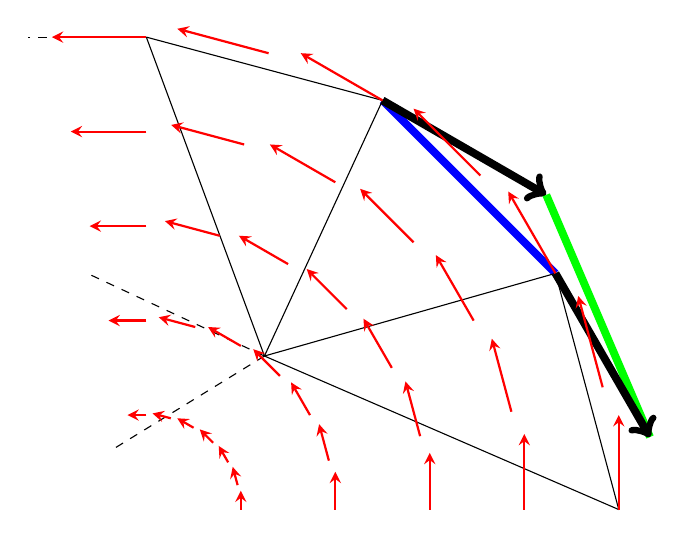
\begin{tikzpicture}[scale=1.5]
  
        \pgfmathsetmacro{\dt}{.4}
        \draw (4,0) --  (3.4641,2);
        \draw[blue,line width=1mm] (3.4641,2) -- (2,3.4641) ;
        \draw[->,line width=1mm] (2,3.4641) -- (2+\dt*3.4641,3.4641-\dt*2);
        \draw[green,line width=1mm] (2+\dt*3.4641,3.4641-\dt*2) -- (3.4641+\dt*2,2-\dt*3.4641);
        \draw[->,line width=1mm] (3.4641,2) -- (3.4641+\dt*2,2-\dt*3.4641);
        \draw (3.4641,2) -- (1,1.3) -- (2,3.4641) ;
        \draw (0,4) -- (1,1.3) -- (4,0) ;
        \draw (2,3.4641) -- (0,4) ;
        \draw[dashed] (0,4) -- (-1,4) ;
        \draw[dashed] (1,1.3) -- (-.5,2);
        \draw[dashed] (1,1.3) -- (-.3,.5);
        \pgfmathsetmacro{\deltaAngle}{15}
        \foreach \radius in {.2,.4,...,1}{
        \foreach \angle in {0,\deltaAngle,...,100}{
            
            
            \pgfmathsetmacro{\scale}{.2}
            \pgfmathsetmacro{\CosValueBase}{\radius*4*cos(\angle)}
            \pgfmathsetmacro{\SinValueBase}{\radius*4*sin(\angle)}
            \pgfmathsetmacro{\CosValueVec}{\CosValueBase-\scale*\SinValueBase}
            \pgfmathsetmacro{\SinValueVec}{\SinValueBase+\scale*\CosValueBase}
           
            
            \draw[-stealth, thick, red]  (\CosValueBase,\SinValueBase) -- (\CosValueVec,\SinValueVec);
        
        }
        }
  \end{tikzpicture}

\end{document}